\subsection{Scene Graph\label{SceneGraph}}

%\begin{figure*}[htb]
\begin{center}
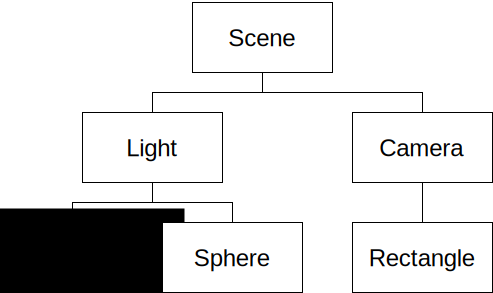
\includegraphics[width=7cm]{media/scene.pdf}
%\caption{A diagram of a possible scene graph.\label{imgScene}}
\end{center}
%\end{figure*}

\paragraph{}
The scene graph is organized by state.
State modifying containers contain visual objects.
The scene is a special container.

\subsubsection{Objects\label{ImplObject}}
Most objects represent a visual shape.
They are organized in an inheritance hierarchy, all based on the class \texttt{Object}.
This hierarchy heavily relies on polymorphism, so there are several virtual member functions that can be customized.

An object offers visibility through drawing itself in \textit{OpenGL} and persistence by writing itself to a stream as lua code.
An objects can also return a smart pointer to itself.
To make this possible, objects should always be wrapped in a \lstinline{shared_ptr}, raw pointers should not be used.
The method \lstinline{clone()} creates an exact deep copy of the object.
For the UI, it can return a dialog that directly changes the parameters of the object.
Other classes can install handlers into an object to be notified when it is modified.

The use and subclassing is described in section \ref{DocObject}.

\paragraph{Primitive Objects}
The sphere, rectangle and parallelepiped object nodes are simple polygon node objects.
They generate parametrized representations with custom subdivision strength.
This is important for lighting, since \textit{OpenGL} only calculates lighting on a vertex basis.

Spheres are generated with the \lstinline{gluQuadric*} functionality.
Rectangles and parallelepipeds are drawn with custom code.

\paragraph{Pixelplane}
Pixel planes are special texture objects.
They have no visual on their own, but draw the associated texture directly into the buffer.
Textures have the ability to draw themselves, so the pixel plane just sets the raster position.
Clipping is done on this position, which will lead to problems when pixel planes are drawn partially off screen.
Solving this is problematic and requires dealing with \textit{OpenGL} internals when manually drawing a subset of the image data.

\paragraph{Mesh}
The mesh node is the most flexible shape node.
It stores a mesh in a simple data structure, and draws this mesh as its visual representation.
The mesh can contain texture and normal values in addition to vertex coordinates.

As input format, Alias Wavefront's Object format is used.
It is parsed by the obj library bundled with \ER.

To accelerate drawing, an \textit{OpenGL} display list is built.
To help drawing of different types of triangles, a small internal wrapper class is used.

\paragraph{Text}
The text node is a shape node that draws text.
It uses Qt's \lstinline{QGLWidget::renderText()} method to draw strings on screen.
This call uses the stencil buffer, so it is incompatible with the line-interlacing renderer that also uses the stencil buffer.

Alternative solutions to render text could include using pre-rendered bitmap letters as textures, or similar approaches.
It should be noted that good text rendering is complicated, modern fonts contain more than just simple letters and spacing data.

\paragraph{}
For more details please refer to the header file (see page \pageref{object.h}) or the doxygen documentation.
For an overview of objects, see section \ref{nodeTypes}.

\subsubsection{Containers\label{ImplContainer}}
\paragraph{}
Container nodes are a special subclass hierarchy of objects.
They can contain any kind of objects, including other containers, and modify how those objects are drawn.
Most nodes modify the \textit{OpenGL} stack, draw their contents and restore the previous stack.

\paragraph{Transformation}
The most used container class is likely \lstinline{AffineTransformation}\cite{affine}.
It encapsulates a 4x4 transformation matrix and convenience accessors to easily modify the transformation.
Since normal shape nodes don't have a rotation property, transformation nodes are used to rotate them.

When a transformation node is drawn, it applies its translation, multiplies its matrix with the transformation matrix on top of the stack and draws its contents.
The original top of the matrix stack is restored after the containing nodes have been drawn.

\paragraph{Light}
For lighting, the class \lstinline{LightNode} is used.
It applies a colored light with ambient light to all contained items.
This only makes sense if those items have normal vectors, since the lighting equation requires them to calculate the litt object color.

For lighting, \textit{OpenGL}'s light model is used.
Not all parameters are exposed, but modifying or extending the class is possible.
Possible extensions could include support for spot light or parallell light sources in addition to the currently implemented point light sources.

The light node enables auto normalisation of vertex normals to compensate for possible scaling or other transformations of objects.
To define the object color easily, the \lstinline{GL_COLOR_MATERIAL} facility is used.
Colored objects automatically use this color as material color.
Due to a limitation in \textit{OpenGL}, only eight lights can be active at a time.
The depth of light nodes contained within other light nodes should therefore not exceed eight.

\paragraph{Fog}
To create atmospheric effects such as smog or fog, the class \lstinline{Atmosphere} is used.
It is a simple wrapper to \textit{OpenGL}'s \lstinline{GL_FOG} facility.
The same three types of foc are supported, and all parameters used by the foc facility can be set.

\paragraph{Camera}
The class \lstinline{CameraNode} is a powerful tool in creating non-consistent scenes.
It projects contained sub-objects with its own camera instead of the scene camera.

It is implemented by loading the internal camera into the projection matrix stack, drawing the contained objects with this camera, and then restoring the original projection.

Due to the limitations of \textit{OpenGL}, the number of recursions is limited by the maximal depth of the projection matrix stack.
Since there is no benefit in recursing camera nodes, users should not do it to prevent problems.

For more information on cameras, see \ref{RendCamera}.

\paragraph{Depth Buffer}
The class \lstinline{DepthBuffer} is the only container subclass that does more than modifying and restoring \textit{OpenGL}'s state.
It clears the depth buffer after every sub object is drawn.
The depth ordering of objects on screen is therefore in draw order.
Object internally, the depth order is still maintained by the depth buffer, so the front- and back-face of objects is maintained.


\subsubsection{Surfaces}
Surfaces are used to place textures on objects.
The simplest surface is \lstinline{Texture}, a simple bitmap texture.
More sophisticated is the family of \lstinline{AbstractStereogram}, bitmap textures that are different depending on the side of the camera they are seen with.

The most prominent subclass is \lstinline{Randomdot-Stereogram}, a random dot texture generated from a depth map (see \ref{Stereogram}).
Other classes offer custom textures in depth-based stereograms, or custom stereograms.

